\section{Actividades de gestión de configuración}
\par A lo largo de este apartado se explicarán las actividades de Gestión de Configuración del Software (SCM) que se van a realizar durante el desarrollo del proyecto CARSEAFTY. Para ello, primero se hará una identificación de la configuración y finalmente se detallará el control de cambios de la configuración.

\subsection{Identificación de la configuración}
\par A continuación se identificará y se hará una descripción detallada de todos aquellos elementos que deban ser considerados Elementos de Configuración (EC).
\subsubsection{Se establece la jerarquía preliminar del producto}
\par En este apartado se estudia y muestra una primera visión de la estructura del sistema software. Esta estructura está definida por sistemas y subsistemas, así como por las relaciones entre cada uno de ellos. En la figura \ref{img:relSys} podemos ver un esquema simplificado de esta estructura.
\par A continuación se describen los sistemas y subsistemas que entran en juego en el sistema software:

\begin{description}[style=multiline, leftmargin=4cm]
  \item[\textbf{Subsistema \textit{pre-crash}:}] este subsistema se encarga del control de posibles colisiones y la disminución de la velocidad o parada del vehículo en caso de alta probabilidad de colisión.
  \item[\textbf{Subsistema de alerta de velocidad:}] este subsistema se encarga de alertar al conductor si la velocidad instantánea del vehículo supera la velocidad máxima permitida en la vía.
  \item[\textbf{Subsistema de control de punto ciego:}] este subsistema se encarga de advertir al conductor de la presencia de vehículos en el lateral trasero del vehículo (en el conocido como punto ciego).
  \item[\textbf{Subsistema de control de la fatiga:}] este subsistema se encarga de avisar al conductor en caso de que este pierda la atención al volante a causa de la fatiga o similar.
  \item[\textbf{Subsistema de cambio de carril:}] este subsistema es el encargado de comparar la trayectoria del vehículo con la de la vía y advertir al conductor si el vehículo se desvía de la trayectoria que debe seguir.
  \item[\textbf{Subsistema de llamada de emergencia:}] este subsistema de encarga de realizar una llamada a los servicios de emergencia en caso de que sea necesario.
  \item[\textbf{Sistema de comunicación central:}] este sistema se encarga de comunicar el resto de subsistemas con el sistema central de CARSEAFTY.
  \item[\textbf{Sistema CARSEAFTY:}] este sistema es el encargado de centralizar la información, mostrarla al conductor y tomar las decisiones sobre las medidas a tomar en cada caso.
\end{description}

\begin{figure}[H]
\begin{center}
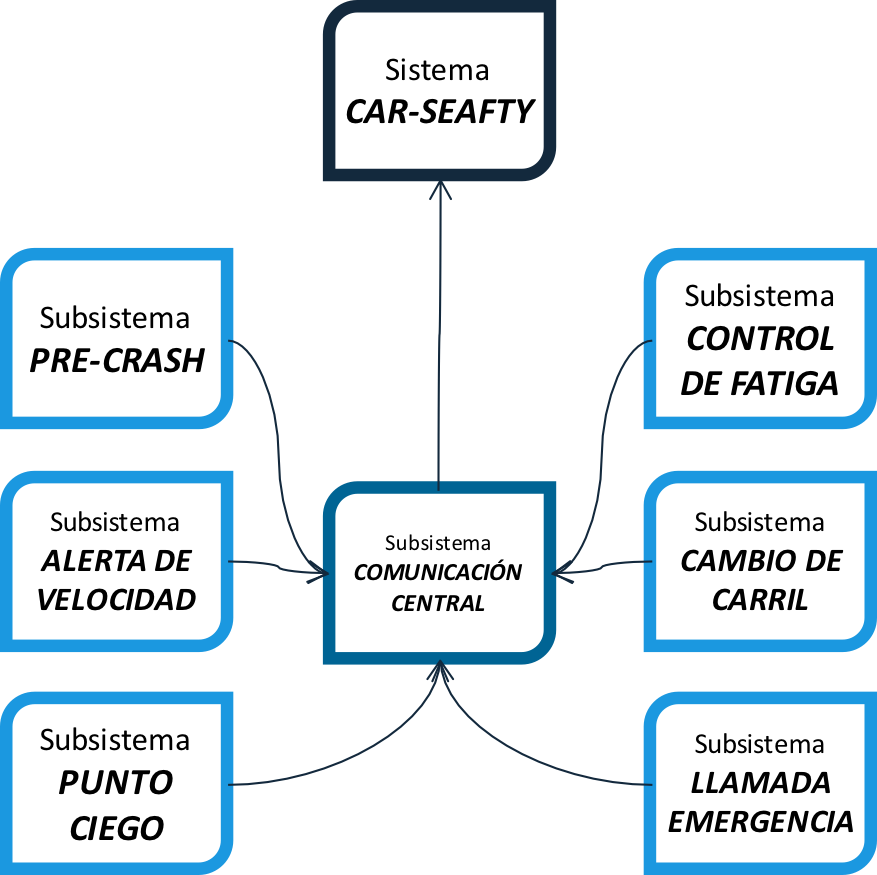
\includegraphics[width=0.8\textwidth]{./img/relSubsystems}
\end{center}
\caption{Estructura de los sistemas y subsistemas}
\label{img:relSys}
\end{figure}



\subsubsection{Selección de los elementos de configuración}
\par En este apartado se identifican los Elementos de Configuración (EC). Éstos son las unidades que se deben poder definir y controlar de forma separada e independiente unos de otros. Así, se corresponden en este proyecto con los productos de las tareas de la metodología de Craig Larman \cite{ART:CraigLarman} y , de forma complementaría, de Métrica3 \cite{WEB:Metrica3}.
\par Pueden verse en la tabla \ref{tab:EC}, en la que se indica el nombre del EC identificado.


\begin{center}
\begin{longtable}{l}

%HEAD
\textbf{NOMBRE} \\\hline \hline
\endfirsthead
\textbf{NOMBRE} \\\hline \hline
\endhead

%FOOT
\hline \multicolumn{1}{r}{\textit{Continúa en la siguiente página}} \\
\endfoot
\endlastfoot

%table
Documento de oferta\\
Documento de control de costes\\
Estudio de Viabilidad del Sistema\\
Plan de Gestión de la Configuración\\
Plan de Calidad\\
Diagrama de casos de uso\\
Matriz de trazabilidad\\
Casos de uso de alto nivel\\
Priorización de casos de uso\\
Casos de uso en formato expandido\\
Arquitectura del sistema\\
Estimación\\
Planificación y seguimiento\\
Modelo de clases\\
Contratos de operación\\
Diagramas de secuencia\\
Gestión de cambios\\
Estándar de implementación\\
Ejecutable de implementación\\
Diagrama de estados\\
Reporte de pruebas\\
Presentación del sistema\\
Informes quinquenales de seguimiento\\\hline

\caption{Elementos de Configuración.}\\
\label{tab:EC}
\end{longtable}
\end{center}


\subsubsection{Selección del esquema de identificación}
\par Tras la identificación de los ECs del apartado anterior, es necesario escoger un esquema de identificación para poder referencialos a lo largo tanto del presente documento como del proyecto.
\par Para ello, hemos decidido usar una identificación no significativa. Los motivos para esta elección se fundamenten en dos aspectos básicos: por un lado, la fácil asignación de código identificativo; en segundo lugar, el uso de un medio electrónico para el desarrollo del proyecto, lo que suple el déficit de la identificación de identificativa. Mediante el uso de hipervínculo se puede referenciar cada uno de los EC a pesar de que su nombre no sea identificativo.
\par Por ello, cada uno de los EC seleccionados en el apartado anterior, sus variantes y versiones serán identificados mediante cuatro dígitos antecedidos por las letras EC.
% \par En la tabla \ref{tab:ECiden} mostramos la tabla \ref{tab:EC} completa, incluyendo el identificador de cada uno de los EC. Se debe tener en cuenta que, en cada iteración, se podrán crear variaciones o modificaciones de los EC, dando lugar a nuevos EC con identificador distinto. An la tabla \ref{tab:ECiden} se muestran los identificadores de los EC en la primera iteración.
%
% \begin{center}
% \begin{longtable}{l l}
%
% %HEAD
% \textbf{NOMBRE} & \textbf{IDENTIFICADOR} \\\hline \hline
% \endfirsthead
% \textbf{NOMBRE} & \textbf{IDENTIFICADOR}\\\hline \hline
% \endhead
%
% %FOOT
% \hline \multicolumn{2}{r}{\textit{Continúa en la siguiente página}} \\
% \endfoot
% \endlastfoot
%
% %table
% \label{EC:0001}Documento de oferta & EC0001\\
% \label{EC:0002}Documento de control de costes & EC0002\\
% \label{EC:0003}Estudio de Viabilidad del Sistema & EC0003\\
% \label{EC:0004}Plan de Gestión de la Configuración & EC0004\\
% \label{EC:0005}Plan de Calidad & EC0005\\
% \label{EC:0006}Diagrama de casos de uso & EC0006\\
% \label{EC:0007}Matriz de trazabilidad & EC0007\\
% \label{EC:0008}Casos de uso de alto nivel & EC0008\\
% \label{EC:0009}Priorización de casos de uso & EC0009\\
% \label{EC:0010}Casos de uso en formato expandido & EC0010\\
% \label{EC:0011}Arquitectura del sistema & EC0011\\
% \label{EC:0012}Estimación & EC0012\\
% \label{EC:0013}Planificación y seguimiento & EC0013\\
% \label{EC:0014}Modelo de clases & EC0014\\
% \label{EC:0015}Contratos de operación & EC0015\\
% \label{EC:0016}Diagramas de secuencia & EC0016\\
% \label{EC:0017}Gestión de cambios & EC0017\\
% \label{EC:0018}Estándar de implementación & EC0018\\
% \label{EC:0019}Ejecutable de implementación & EC0019\\
% \label{EC:0020}Diagrama de estados & EC0020\\
% \label{EC:0021}Reporte de pruebas & EC0021\\
% \label{EC:0022}Presentación del sistema & EC0022\\
% \label{EC:0023}Informes quinquenales de seguimiento & EC0023\\\hline
%
% \caption{Elementos de Configuración identificados.}\\
% \label{tab:ECiden}
% \end{longtable}
% \end{center}

\par Por otro lado, la descripción de los elementos de configuración constará del código identificativo, el nombre del EC, su descripción, la iteración en la que surgió o fue identificado, la fecha de creación y el código identificativo de la línea base. Puede verse un ejemplo de esta tabla descriptiva en la tabla \ref{tab:ECdescription}.

\begin{table}[h]
\begin{center}
\begin{tabular}{ r l | r l }
  \hline
\textbf{Código Identificativo:} & Código & \textbf{Nombre:} & Nombre del EC \\
\textbf{Iteración:} & Iteración & \textbf{Fecha de creación:} & dd/mm/aaaa \\ \hline \hline
\textbf{Descripción:} & \multicolumn{3}{l}{Descripción del EC} \\
\textbf{Línea base:} & \multicolumn{3}{l}{Línea base del EC} \\
\hline
\end{tabular}
\caption{Ejemplo de la Descripción de un EC.}
\label{tab:ECdescription}
\end{center}
\end{table}

\subsubsection{Definición de relaciones}
\par Tras definir los diferentes EC y saber como identificarlos, debemos definir e identificar las relaciones que existen entre ellos. Ello sirve para poder conocer qué elementos de configuración se ven afectados con los posibles cambios de otros elementos de configuración, y así poder delimitar los posibles impactos que se puedan producir.
\par En nuestro proyecto contemplamos varias posibles relaciones:

\begin{description}[style=multiline, leftmargin=4cm]
  \item[\textbf{Dependencia (DEP):}] relación que se da cuando un EC tiene relación directa con otro EC. Es decir, si un EC cambia, el que tenga relación directa con él se verá afectado y podrá resultar modificado.
  \item[\textbf{Derivación (DER):}] relación que se da cuando un EC requiere que haya terminado otro anterior.
  \item[\textbf{Sucesión (SUC):}] relación de histórico de cambios sobre un EC de una revisión a otra.
  \item[\textbf{Variante (VAR):}] relación de las distintas variaciones que hay sobre un mismo EC.
  \item[\textbf{Composición (COMP):}] relación que se da cuando un EC está compuesto por un conjunto de ECs.
\end{description}

\par Una vez vistas las distintas relaciones que se pueden dar entre dos EC, pasamos a proponer un esquema de identificación de las mismas. Lo primero que se indicará, tal y como se ve en la figura \ref{img:relEC}, serán los identificadores de los dos EC relacionados separados por un guión. A continuación, y mediante la separación por otro guión, se indicará la abreviatura de la relación que los uno vista en el párrafo anterior.

\begin{figure}[hb]
\begin{center}

\includegraphics[width=0.8\textwidth]{./img/relEC}
\end{center}
\caption{Esquema de identificación de relación entre ECs.}
\label{img:relEC}
\end{figure}

\par En cuanto a las relaciones y al esquema mencionado, se deben tener varios aspectos en cuenta:
\begin{itemize}[-]
  \item Si la relación es bidireccional (véase Relación de Dependencia), el orden de los identificadores que se indique en es esquema de la figura \ref{img:relEC} es indiferente.
  \item Si la relación es unidireccional, el orden de los elementos de configuración en el formato sí es significativo. En la Relación de Derivación (DER), EC1-EC2-DER implica que EC2 deriva de EC1. En el caso de la Relación de Sucesión (SUC), EC1-EC2-SUC implica que EC2 surge de una revisión de EC1, por lo que EC2 es el \textit{hijo} de EC1.
  \item Si la relación es de Composición (COMP), se añadirán tantos identificadores como sean necesarios al esquema de la figura \ref{img:relEC}, siendo EC1 el EC que se compone de los EC2 a ECn.
  \item Si la relación es de Sucesión (SUC), EC1-EC2-SUC implica que EC1 es una versión actualizada de EC2. Véase que al ser un identificador no significativo, cada versión de un mismo EC tiene un identificador distinto.
  \item SI la relación es Variante (VAR), EC1-EC2-VAR implica que EC2 es una variante de EC1.
\end{itemize}



\subsubsection{Definición y establecimiento de líneas base}
\par En este apartado se recogen las diferentes líneas base del proyecto. Como se puede ver en la tabla \ref{tab:baseLine} para cada una de ellas recogemos su nombre, su descripción, su estado (que será o bien \textit{abierta} o bien \textit{cerrada}), la fecha y los identificadores de los EC que la componen.

\begin{table}[h]
\begin{center}
\begin{tabular}{ r l | r l }
\hline
\textbf{Nombre:} & \multicolumn{3}{l}{Nombre de la línea base} \\
\textbf{Descripción:} & \multicolumn{3}{l}{Descripción de la línea base} \\ \hline \hline
\textbf{Estado:} & Abierta/Cerrada & \textbf{Fecha de creación:} & dd/mm/aaaa \\
\textbf{EC1} & Identificador EC1 & \textbf{EC2} & Identificador EC2 \\
\textbf{EC3} & Identificador EC3 & \textbf{ECn} & Identificador ECn \\
\hline
\end{tabular}
\caption{Ejemplo de una Línea Base.}
\label{tab:baseLine}
\end{center}
\end{table}

\par Las líneas base definidas en este proyecto son:
\begin{itemize}[-]
  \item Fase de Documentación
  \item Fase de Planificación y Especificación de requisitos
  \item Fase de Análisis de la primera iteración
  \item Fase de Diseño de la primera iteración
  \item Fase de Análisis de la segunda iteración
  \item Fase de Diseño de la segunda iteración
  \item Fase de Análisis de la tercera iteración
  \item Fase de Diseño de la tercera iteración
  \item Fase de Implementación
\end{itemize}


\subsubsection{Definición y establecimiento de bibliotecas de software}
\par A lo largo de este apartado se definirán las bibliotecas de software que serán usadas durante el proyecto. Así mismo, se establecerá su ubicación exacta dentro del proyecto. Así, y como se verá en este apartado, incluiremos bibliotecas de documentación, de soporte, de desarrollo, de \textit{backup} y una maestra, entre otras.
\par Así, las bibliotecas establecidas se ubicarán todas ellas dentro de la siguiente ruta:
\begin{lstlisting}
   $PATH:$ /User/carseafty/
\end{lstlisting}

\par Puede verse un esquema del sistema de librerías en la figura \ref{img:softwareLibrary}. Las bibliotecas de nuestro proyecto serán:

\begin{description}[style=multiline, leftmargin=4cm]

  \item[\textbf{Documentación:}] contendrá la documentación del proyecto. Esta documentación estará recogida en cuatro subgrupos diferentes: la documentación relativa a la oferta y los costes, la documentación de Estudio de Viabilidad del Sistema, la documentación de calidad y la documentación de configuración.
  \par La ubicación de cada una de estas carpetas será:
  \begin{lstlisting}
     $PATH:$ /User/carseafty/documentation/offer
     $PATH:$ /User/carseafty/documentation/evs
     $PATH:$ /User/carseafty/documentation/quality
     $PATH:$ /User/carseafty/documentation/configuration
  \end{lstlisting}

  \item[\textbf{Desarrollo:}] esta biblioteca recoge el trabajo desarrollado por el equipo de desarrollo. El código y documentación aquí almacenado está en proceso, pero no acabado. Una vez estén finalizados, pasarán a la biblioteca de producción. Esta biblioteca está dividida en las siguientes bibliotecas, correspondientes a los subsistemas del proyecto:
  \begin{lstlisting}
     $PATH:$ /User/carseafty/development/precrash
     $PATH:$ /User/carseafty/development/velocity
     $PATH:$ /User/carseafty/development/laneChange
     $PATH:$ /User/carseafty/development/blindSpot
     $PATH:$ /User/carseafty/development/ecall
     $PATH:$ /User/carseafty/development/fatigue
     $PATH:$ /User/carseafty/development/comunication
  \end{lstlisting}

  \item[\textbf{Producción:}] esta biblioteca contiene las líneas base creadas y acabadas. La ubicación exacta es:
  \begin{lstlisting}
     $PATH:$ /User/carseafty/production
  \end{lstlisting}

  \item[\textbf{Maestra:}] esta biblioteca contiene la versión actual del cliente. La ubicación exacta es:
  \begin{lstlisting}
     $PATH:$ /User/carseafty/production/master
  \end{lstlisting}

  \item[\textbf{Proves:}] esta carpeta contiene las pruebas realizadas sobre las distintas versiones del proyecto. Cada una de las versiones probadas tendrá una subcarpeta dentro de:
  \begin{lstlisting}
     $PATH:$ /User/carseafty/proves
  \end{lstlisting}

  \item[\textbf{Backup:}] almacena una copia de seguridad. La ubicación exacta es:
  \begin{lstlisting}
     $PATH:$ /User/carseafty/buckup
  \end{lstlisting}

\end{description}

\par Como se indicó en al apartado \ref{subsec:politics}, se utilizará BitBucket para el almacenamiento de la documentación y el código. Así, se especificarán los permisos de cada una de las bibliotecas en función de la tabla \ref{tab:bibAdmin}. Cabe destacar que si un miembro del equipo tiene permisos sobre una biblioteca de nivel superior, ello implica que tiene permisos sobre todas las bibliotecas de niveles inferiores.

% \begin{table}[h]
% \begin{center}
% \begin{tabular}{ p{5cm} | r }
% \hline
% 	\textbf{Responsable} & \textbf{Ocupación} \\ \hline \hline
%   Juan Abascal & SCMR \\
%   Adriana Lima & CC \\
%   Alberto García & Bibliotecario \\
%   Carlos Olivares Sanchez-Manjavacas, Carlos Tormo Sánchez, Irina Shayk & Equipo de desarrollo \\ \hline
% \end{tabular}
% \caption{Responsabilidades.}
% \label{tab:bibAdmin}
% \end{center}
% \end{table}



\subsection{Control de cambios en la configuración}
\subsubsection{Procedimiento aplicable}
\par A lo largo de esta sección detallamos las actividades de solicitud, evaluación, aprobación e implementación de los cambios solicitados y realizados en los elementos de la configuración. El procedimiento descrito a continuación es el que se utilizará cada vez que se precise introducir un cambio en el sistema.
\par Este proceso se describe en la figura \ref{img:planAprobCambios}. Atendiendo a la misma, los pasos que se deben seguir son los siguientes:

\begin{figure}[hb]
\begin{center}
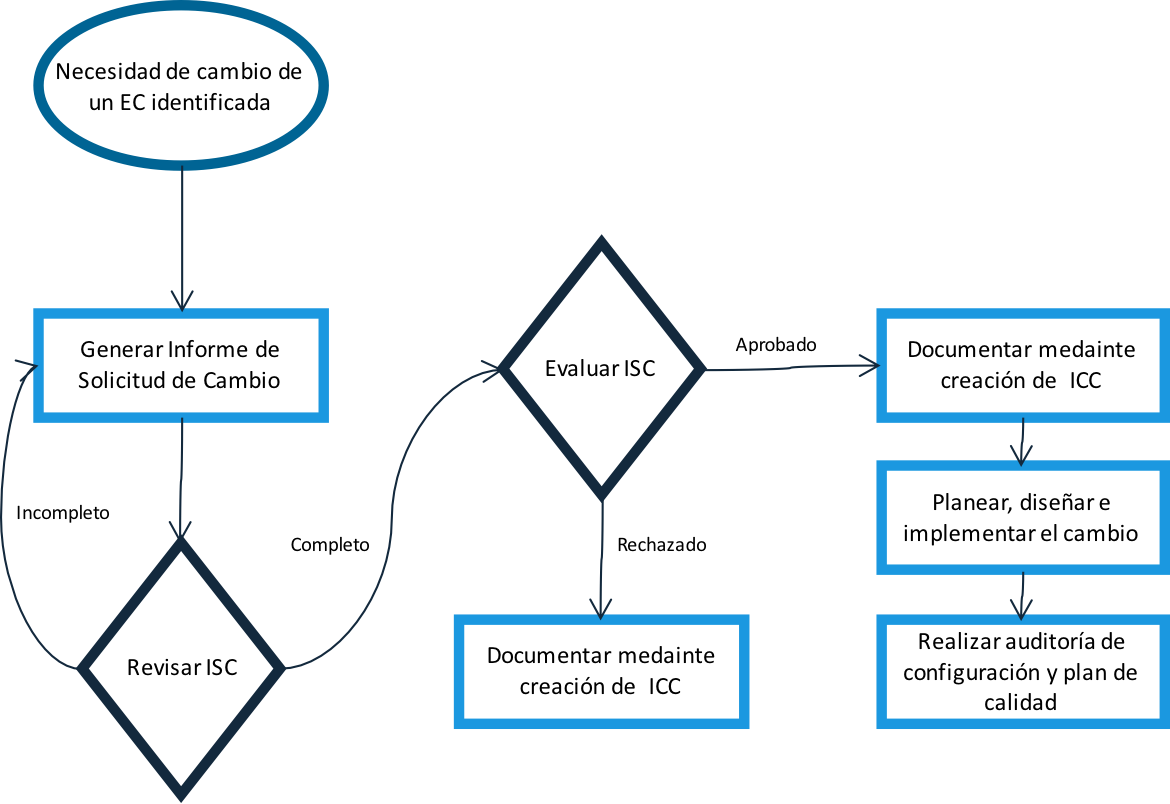
\includegraphics[width=1\textwidth]{./img/planAprobacion}
\end{center}
\caption{Procedimiento General de Control de Cambios.}
\label{img:planAprobCambios}
\end{figure}

\begin{enumerate}

  \item Cuando un posible cambio en un EC es identificado, se debe generar una instancia del Informe de Solicitud de Cambios (véase \ref{inf:ISC}). Este debe recoger toda la información necesaria para justificar dicho cambio. Así mismo, es necesario que sea lo más detallado posible. Este informe será colocado en la carpeta de \textit{configuration}, dentro de la carpeta de \textit{changes} y, más concretamente, en la subcarpeta de \textit{inProgress}. La ruta concreta sería:
  \begin{lstlisting}
     $PATH:$ /User/carseafty/documentation/configuration/changes/inProgress
  \end{lstlisting}

  \item Una vez realizado el Informe de Solicitud de Cambio y registrada la petición, se debe revisar si esta está completa o no. Esta revisión será en parte prescindible si el formulario es electrónico y no permite el envío del mismo en caso de estar incompleto. Tras realizar esta comprobación, se debe evaluar la solicitud. Esta evaluación debe tener en cuenta los ECs afectados y el posible impacto de los cambios solicitados. Así, el Comité de Control de la Configuración debe decidir si aceptar o no la petición correspondiente.

  \item En caso de que el CGC decida rechazar el cambio, la petición (el ISC) deberá ser trasladado a la carpeta:
  \begin{lstlisting}
     $MOVE TO:$ /User/carseafty/documentation/configuration/changes/evaluated
  \end{lstlisting}
  Además, se creará un Informa de Certificación de Cambios que se almacenará en la misma carpeta indicando el motivo de la denegación.

  \item En caso de que el CGC decida aceptar la petición, deberá redactarse el ICC, indicando los aspectos antes detallados, y se almacenaráen la carpeta:
  \begin{lstlisting}
     $PATH:$ /User/carseafty/documentation/configuration/changes/inProgress
  \end{lstlisting}

  \item A continuación, si el cambio ha sido aceptado, se debe diseñar y planificar el cambio para decidir cuándo llevar a caso su implementación. Dicha implementación será ejercida tanto en el elemento de la configuración sobre el que se solicitó el cambio como en los EC que estén relacionados con éste y cuyo cambio afecte.

  \item Una vez el cambio sea realizado, se moverán ambos archivos (el ICC correspondiente y el ISC del cambio aplicado) a la carpeta:
  \begin{lstlisting}
     $MOVE TO:$ /User/carseafty/documentation/configuration/changes/evaluated
  \end{lstlisting}

\end{enumerate}


\subsubsection{Formato del Informe de Solicitud de Cambios}\label{inf:ISC}
Puede encontrarse el Informe de Solicitud de Cambios en esta URL: https://carlososm.typeform.com/to/cuwCDI.
\subsubsection{Formato del Informe de Certificación de Cambios}
Puede encontrarse el Informe de Certificación de Cambios en esta URL: https://carlososm.typeform.com/to/DVPDc6.


\begin{figure}[hb]
\begin{center}
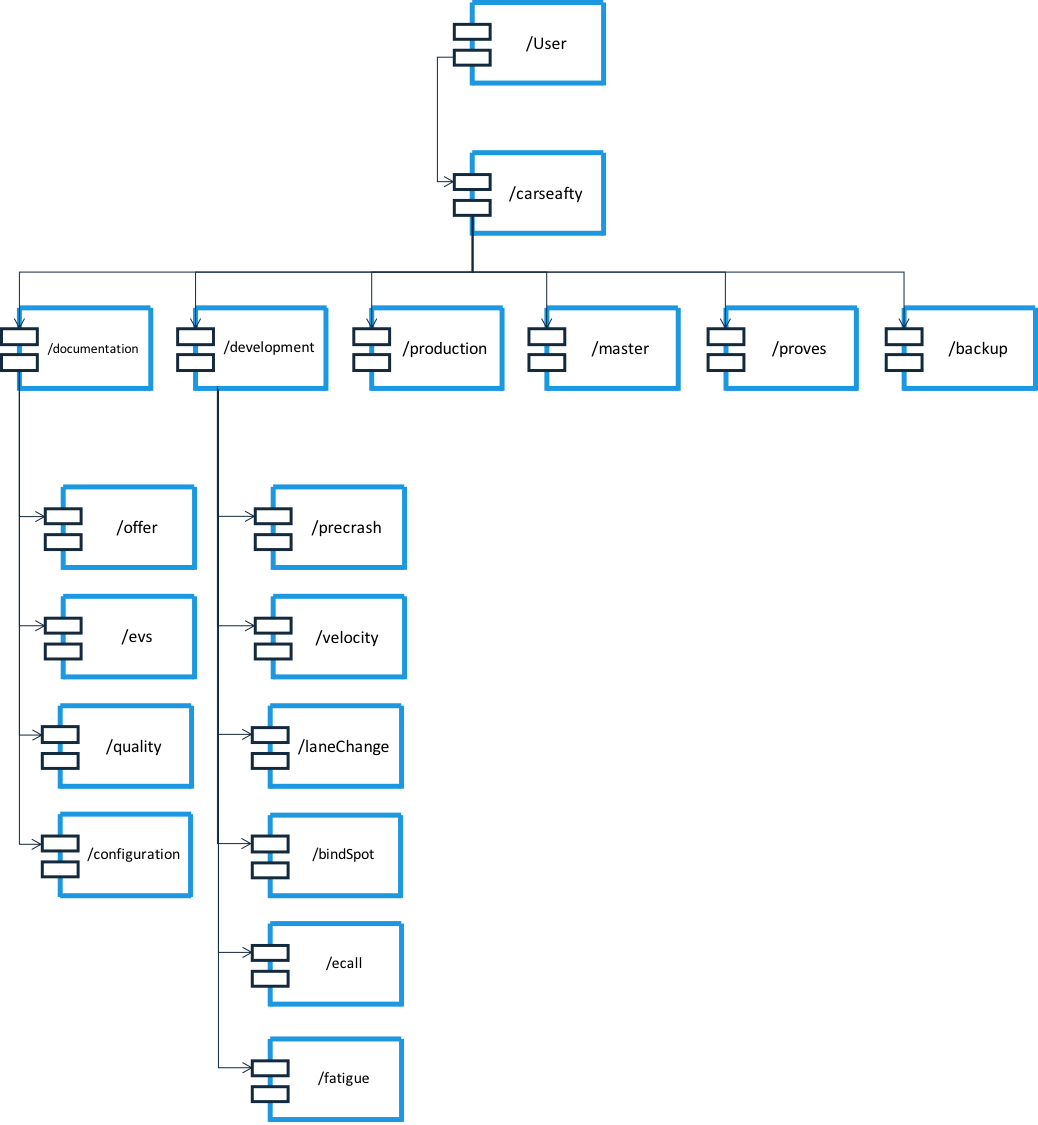
\includegraphics[width=1\textwidth]{./img/softwareLibrary}
\end{center}
\caption{Esquema de identificación de relación entre ECs.}
\label{img:softwareLibrary}
\end{figure}
